\chapter{二次記憶装置}

容量が小さく揮発性の主記憶だけでは
コンピュータを実用的に使用することができない.
大容量で不揮発性の二次記憶装置を
プログラムやデータを格納したファイルの永続的な置き場として使用する.
ファイルを永続的に記憶するためには,
大容量で不揮発性の二次記憶装置が適している.

%==============================================================================
\section{記憶装置の階層}
現代のコンピュータは,様々な種類の記憶装置を使用している.
\figref{memoryHierachy}にコンピュータの記憶装置の関係を簡単に示す.
図では,上の層にあるものほど高価で高速なメモリである.

\begin{enumerate}
\item \emph{レジスタ}はCPUレジスタのことを表す.
  CPUレジスタは容量が小さい\footnote{多くのCPUでは数十バイト程度である.}が
  高速にアクセスすることが可能な記憶装置である.

\item \emph{主記憶(メモリ)}は数ナノ秒〜十数ナノ秒程度の
  時間でアクセスできる高速な記憶装置である.
  コンピュータはプログラムやデータを主記憶にロードして実行する.
  主記憶の容量は数Giバイト〜数十Giバイト程度であり,
  オペレーティングシステムと全てアプリケーションを格納すには小さすぎる.

\item \emph{二次記憶装置}は,
  近年では,ハードディスクやSSD(Solid State Drive)のことである.
  容量は大きいが,主記憶と比べるとアクセス時間がとても遅い\footnote{
    ハードディスクの場合だと数ミリ秒〜数十ミリ秒もかかる.}.
  しかし,2次記憶装置には電源を切ってもデータが消えない特性がある\footnote{
    ハードディスクなら磁気的に記録しているので消えない.
    SSDならフラッシュメモリに記録しているので消えない.}.
  この特性は不揮発性と呼ばれる.
\end{enumerate}

\myfigure{btp}{scale=1.6}{Fig/memoryHierarchy.pdf}{記憶の階層}{memoryHierachy}

各記憶装置には以上のような特性があるので,
夫々の特性に合った使い方をする必要がある.
オペレーティングシステム,アプリケーションプログラム,
データの全てを永続的に格納するには,
\emph{大容量で不揮発性の二次記憶装置}が適している.

%==============================================================================
\section{二次記憶装置の種類}
接続方式と記憶媒体によって分類できる.

\subsection{接続方式}
\figref{hardBlockAgain}に示すように,
主記憶はCPUとバスによって直接に接続される.
一方で二次記憶装置はホストコントローラ配下の外部バスに接続されることが多い.
CPUとホストコントローラはバスによって接続される.
ホストコントローラから先はUSBやSATAのような外部バスである.
二次記憶装置はUSBやSATAバスの先に接続される.
このように二次記憶装置は,
CPUから直接アクセスすることはできない.

\myfigure{btp}{scale=0.55}{Fig/hardBlock-crop.pdf}
         {ハードウエア構成(再掲)}{hardBlockAgain}

USBバスに接続されたメモリスティックやハードディスクは,
PC稼働中に接続・取り外しが可能である.
また,CD-ROMなどの光ディスクも取り外し可能である.
これらは,データ交換用やバックアップ用に都合が良い.

\subsection{記憶媒体による分類}
二次記憶装置は大きくテープ型の装置とディスク型の装置に分類できる.
テープ型装置はデータのバックアップやデータの輸送用に用いられてきたが,
最近では使用されることが少なくなっている.
ハードディスクに代表されるディスク型装置は
最もよく使用される二次記憶装置である.
%オペレーティングシステムはハードディスクにインストールされ,
%コンピュータはハードディスクからオペレーティングシステムを読出して起動する.

\begin{enumerate}
\item \emph{テープ型装置}\\
\figref{magneticTape}に磁気テープの写真を示す\footnote{
様々な磁気テープが用いられてきたが最近見かけることが少なくなっている.
写真は,デジタルデータ記録用の8mm磁気テープである.
\figref{hardBlockAgain}に磁気テープを示してないのは
最近見かけなくなったためである.
}.
カセットの中に1本の長いテープが巻き取られた状態で入っている.
データは磁気的にテープに記録される.
データは先頭から順に(シーケンシャルに)書込むことしかできない.
読出す場合も先頭から順に読出すことしかできない.

\emph{シーケンシャルアクセス}しかできないため
読出すデータの位置まで進むために数分かかることもある.
しかし,一度,データの転送が始まるとハードディスク並のデータ転送速度になる.
一般に記録できるデータあたりのメディア(磁気テープ)の値段が安いので,
滅多に使用することが無いバックアップデータを保存するために用いられてきた.

\myfigure{btp}{scale=0.3}{Fig/magneticTape.jpg}{磁気テープ}{magneticTape}

\item \emph{ディスク型装置} \\
ディスク型装置の代表はハードディスクである.
\figref{hardDisk}に蓋を開けた状態のハードディスクの写真を示す\footnote{
3.5インチのハードディスクの蓋を開けた状態である.
普通,蓋を開けるとハードディスクは壊れるので,
写真のハードディスクはこわれている.}.
写真のハードディスクは4枚の円盤が重ねてあり,
各円盤の表裏(合計8面)にデータが記録できる.
データは回転する円盤上に磁気的に記録される.

ディスク型装置の最大の特長は,
データブロックのアドレスを指定して途中からでも自由に読み書きできることである.
このようなアクセスの仕方は\emph{ランダムアクセス}と呼ばれる.
フロッピーディスク,
CD-ROM,
DVD-ROM,
Blu-Ray Disk 等も円盤にデータを記録する方式なのでディスク型装置である.
一方で,SSDや,USBメモリ,メモリカードは円盤にデータを記録する方式では無いが,
ランダムアクセスが可能でハードディスクと同様に扱うことができる.
そのため,
ほとんどのオペレーティングシステムは,これらもディスク型装置として扱う.

\myfigure{btp}{scale=0.3}{Fig/hardDisk.jpg}{ハードディスク}{hardDisk}

\end{enumerate}

%==============================================================================
\section{ハードディスク}
ハードディスクは,
システムの起動ドライブとして使用される.
システム起動後も,
オペレーティングシステムの追加モジュールや
アプリケーションはハードディスクから読み込まれるし,
仮想記憶システムがバッキングストアとしても使用する.
また,アプリケーションがデータを格納する場合も,
まず,第一にハードディスクが選択される.

このようにハードディスクが最も頻繁に使用されるので,
ハードディスクを上手く管理できるかどうかにより,
オペレーティングシステムの性能や使い勝手は大きく左右される.
そのためファイル管理機構はハードディスクを管理することを前提にしている.
また,ハードディスク以外のディスク型装置は
ハードディスクと同様に扱えるように作ってある.
そこで,ハードディスクについて少しだけ詳しく解説する.

\subsection{セクタ・トラック・シリンダ}
回転する円盤に同心円の\emph{トラック}を作り磁気的にデータを記録する.
一周のトラックに記録できるデータは大きすぎるので,
トラックを幾つかのブロックに分割する.
このブロック(サイズは512Bか4KiB)のことを\emph{セクタ}と呼ぶ.
データの読み書きはセクタ単位で行われる.
同じ半径のトラックは円盤の面の数だけ存在することになる.
各円盤面に散らばった同じ半径のトラックを集めたものを\emph{シリンダ}と呼ぶ.

PC用のハードディスクが世の中に出てきた最初から
セクタのサイズは512バイトであった.
そのため,セクタサイズが512バイトと決めつけて最適化している
オペレーティングシステムも存在する.
しかし,ハードディスクの大容量化に伴い2009年頃からセクタサイズを4Kiバイトに
した製品が出回るようになってきた.
最近のオペレーティングシステムは
セクタサイズが512バイト以外でも効率よく働くように改良されている.

\subsection{セクタのアドレッシング}
ハードディスク上の特定のセクタを指定するために,
以下の二つの方式のどちらかが使用される.

\begin{description}
\item[CHS(Cylinder Head Sector)]
  シリンダ番号,トラック番号,セクタ番号の組で1つのセクタを特定できる.
  長い間,ハードディスクの読み書きは,
  これら3つの番号を使用したセクタアドレスを用いて行われてきた.
  PCではトラックをトラックに対応する読み書き\emph{ヘッド}で置換え
  シリンダ(Cylinder),ヘッド(Head),セクタ(Sector)の組で
  セクタアドレスを表現してきた.
  このセクタアドレスの表現方式をCHSと呼ぶ.
\item[LBA(Logical Block Addressing)]
  本来ハードディスクのセクタアドレスは,
  ハードディスクの物理構造を反映した
  シリンダ番号,トラック番号,セクタ番号の組で表すものである.
  オペレーティングシステムは,
  同一ファイルのデータをなるべく同じシリンダに置くなどして,
  ファイルアクセスの効率化を行っていた.
  しかし,現代のハードディスクはブラックボックスになってしまった.
  ディスクコントローラにハードディスクの構造を問い合わせても嘘の情報が
  返されるようになったのである\footnote{
    ディスクの容量を大きすくるために
    外側トラックのセクタ数を内側トラックより多くするなど,
    従来の考え方では表現できない物理構造になってしまった等の事情がある.}.
  そのため,従来の3次元のアドレッシングは煩雑なだけになってしまった.
  現在では全てのセクタに通し番号(1次元のセクタアドレス)をふり,
  この番号でセクタを指定するアドレッシングが一般的である.
  このアドレッシングをLBA方式と呼ぶ.
\end{description}

\subsection{LBA方式のデバイスドライバ例}
TaCがハードディスクの代替として使用するuSDカードの
ホストコントローラはLBA方式を用いて読み書きする.
リスト\ref{tacosReadSct}にLBA方式でディスク型装置を動作させる
TacOSのデイバイスドライバの例を示す.
このリストでは初期化ルーチンは省略している\footnote{
デバイスドライバの全体は
\url{https://github.com/tctsigemura/TacOS/blob/master/os/fs/mmcspi.cmm}
で参照できる.}.
初期化ルーチンは,
このデバイスドライバ専用のセマフォを一つ割り当てた後,
割り込みハンドラを割り込みベクタへ登録するものである.

\lstinputlisting[numbers=left,float=btp,label=tacosReadSct
  ,caption=ディスク型装置のデバイスドライバ例]{Lst/tacosReadSct.cmm}

\begin{description}
\item[\texttt{restart()}関数]
  4行はディスクコントローラの割り込みハンドラである.
  5行の\|semV()|はセマフォのV操作を行う(\figref{tacosSemV}参照).
  割り込み発生時にセマフォを待ち合わせている
  プロセス(ファイルシステムサーバ)を起床させる.
\item[\texttt{readSct()}関数] 12行はデバイスドライバの
  セクタ読み出しルーチンである.
  セクタのアドレスはLBA方式で,
  上位16bit(\|h|)と下位16bit(\|l|)とに分けて渡される.
  \|buf|はデータを読み出すバッファである.
  \|out()|は,アドレスを指定して16bitデータをI/Oポートに出力する関数である.
  13行でバッファのアドレスを
  ディスクコントローラのアドレスレジスタ(\|MEM_ADDR|)に書き込む.
    14,15行でLBAをディスクコントローラのレジスタに書き込み,
    16行でディスクコントローラの動作を開始させる.
    ディスクコントローラがDMA(\pageref{dma}ページ参照)を用いて,
    CPUの力を借りることなく目的のデータをメモリに転送する.
    その間,デバイスドライバを呼び出したプロセス(ファイルシステムサーバ)は
    17行でCPUを解放して割り込みを待つ.
\end{description}

\section{フォーマッティング}
二次記憶装置の使用を開始する前に,
記憶媒体を初期化する必要がある\footnote{
USBメモリやポータブルハードディスクは
初期化済みの状態で販売されている場合が多い.
ほとんどの場合,PCは内蔵ハードディスクを初期化した上で
オペレーティングシステムをインストールした状態で販売されている.
}.
ハードディスクを例に初期化の手順を以下に示す.

\begin{enumerate}
\item \emph{低レベルのフォーマッティング(物理フォーマット)を行う.}\\
  低レベルのフォーマッティングは
  ディスクの表面にトラックを磁気的に描いていく作業である.
  20年以上以前の製品ではユーザが行うことが可能であったが,
  最近は製造時に工場で物理フォーマットを行いユーザにさせない.
%  ディスクコントローラに低レベルフォーマッティングのコマンドを送っても
%  何もしない製品が多い.
\item \emph{必要に応じてディスクをパーティション(区画)に分割する.}\\
  ディスク全体を一つのボリューム\footnote{
    Windowsの用語ではドライブと呼ぶ.}として使用しても良いが,
  システム領域とユーザ領域のように分けて使用したい場合や,
  一台のディスクに複数のオペレーティングシステムを
  インストールする場合は分割する必要がある.
% 分割すると「ユーザデータのみバックアップを取る」等の作業がやりやすくなる.

  \begin{figure}[btp]
    \begin{center}
      \begin{minipage}{0.49\columnwidth}
        \centerline{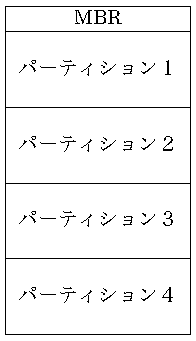
\includegraphics[scale=1.0]{Fig/hddPartition.pdf}}
        \caption{ハードディスクのパーティション}\label{fig:hddPartition}
      \end{minipage}
      \begin{minipage}{0.49\columnwidth}
        \centerline{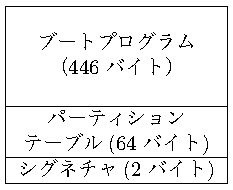
\includegraphics[scale=1.0]{Fig/masterBootRecord.pdf}}
        \caption{PCのMBR(合計512バイト)}\label{fig:masterBootRecord}
      \end{minipage}
    \end{center}
  \end{figure}

 \figref{hddPartition}に4つのパーティションに分割したハードディスクの
  内部を示す\footnote{この例はPCでMBR方式を使用した場合のものである.}.
  \emph{MBR(Master Boot Record)}は,
  ハードディスクの最初のセクタ(LBA0)に格納され,
  ブートプログラムとパーティションテーブルを記録する.
  \figref{masterBootRecord}にMBRの内容を簡単に示す.
  パーティションテーブルに各パーティションの位置と大きさ等が記録される.
  シグネチャはハードディスクが初期化済みかどうかを表すデータである.
  この2バイトに\texttt{55H} \texttt{AAH}が書き込まれていれば,
  初期化済みである.
  
  \myfigure{btp}{scale=1.0}{Fig/partitionTable.pdf}
           {パーティションテーブルの例}{partitionTable}

  パーティションテーブルの例を\figref{partitionTable}に示す.
  この例は,最初に2つパーティションが存在し(\texttt{Flag=80H}),
  残りのエントリは使用されていない(\texttt{Flag=00H})場合を示している.
  図中の\texttt{???}等はフラグによって無効にされたエントリの内容か,
  CHSで表現した値が格納される部分である.
  CHS表現は煩雑になるので省略した.

  パティションテーブルエントリの内容は
  \tabref{partitionTableEntry}の通りである.
  一つのエントリは16バイトの大きさになる.
  \|Type|フィールドの意味は\tabref{partitionTableType}の通りである.
  ここに示したものは一部である\footnote{
    詳しくは''Partition type'',
    \url{https://en.wikipedia.org/wiki/Partition_type}等を参照のこと.}.

  \begin{table}[btp]
    \begin{center}
      \begin{minipage}{0.64\columnwidth}
        \caption{パーティションテーブルのエントリ}
        \label{tab:partitionTableEntry}
        \centerline{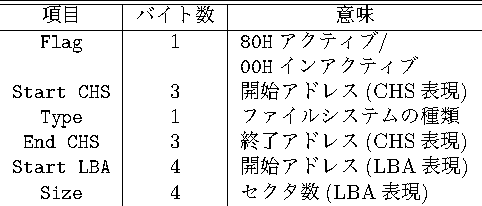
\includegraphics[scale=1.0]{Tbl/partitionTableEntry.pdf}}
      \end{minipage}
      \begin{minipage}{0.34\columnwidth}
        \caption{Typeフィールドの意味}
        \label{tab:partitionTableType}
        \centerline{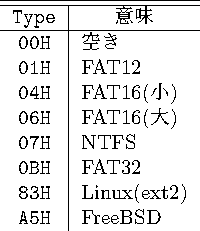
\includegraphics[scale=1.0]{Tbl/partitionTableType.pdf}}
      \end{minipage}
    \end{center}
  \end{table}

\item \emph{論理フォーマッティングを行う.}\\
  論理フォーマッティングは,
  ボリューム(パーティション)に空の状態のファイルシステムを作る作業である.
  空のファイルシステムを表現する管理データをディスクに書込む.
\end{enumerate}

\section{パーティションを見つけるプログラムの例}
パーティションテーブルから
ブート可能なパーティションを見つけるプログラムの例として,
TacOSの\|readMBR()|関数\footnote{\texttt{readMBR()}は
  \url{https://github.com/tctsigemura/TacOS/blob/master/os/fs/blkFile.cmm}
  に含まれる.}
をリスト\ref{tacosReadMBR}に示す.

\lstinputlisting[numbers=left,float=btp,label=tacosReadMBR,
  caption=MBRを解析しアクティブなFAT16パーティションの開始LBAを求める例]
                {Lst/tacosReadMBR.cmm}

\begin{description}
\item[1行] \texttt{bpbLba}は32ビットのLBAを格納するための配列である.
  TaCは16ビットデータしか扱えないので,配列を用いて32ビットデータを格納する.
\item[3行] \texttt{readMBR()}関数は
  \texttt{bpbLba}にブート可能なFAT16パーティションの開始LBAを格納する.
\item[4行] \texttt{buf}に512バイトのメモリ領域を確保する.
\item[5行] 前出の\|readSct()|関数を用いて\|buf|にMBRを読み込む.
\item[7行] MBRの第446バイトからパーティションテーブルが始まる.
  パーティションテーブルエントリのサイズは16バイトである.
\item[8行] エントリの先頭の\|Flag|を読む.
  \|ord()|は\cmm 言語の型変換演算子(文字型から整数型へ変換)である.
\item[9行] エントリの4バイト目の\|Type|を読む.
\item[11行] TacOSはFAT16パーティションにインストールされているので探す.
\item[12行] \|ld32()|は16ビットデータ2個を配列に書き込むマクロ,
  \|wordLE()|は文字配列の指定位置からリトルエンディアンの16ビットデータを
  読み出すマクロである.
  パーティションテーブルエントリから4バイトの\|Start LBA|を読み出して,
  \|bpbLba|に格納している.
\item[13,14行] FAT16パーティションを見つけたのでバッファを解放して終了する.
\end{description}

\section{ブートストラップ}
通常オペレーティングシステムは
コンピュータに内蔵されたハードディスクにインストールされている.
オペレーティングシステムが動作を開始するためには,
何らかの方法でハードディスクから
オペレーティングシステムを主記憶にロードし実行を開始する必要がある.
この作業をブートストラップ(略してブート)と呼ぶ.

多くの場合オペレーティングシステム本体(カーネル)は
ファイルシステム上にファイルとして格納されている.
つまり,これから起動するオペレーティングシステムの
ファイルシステムの構造を解釈し,
カーネルファイルを見つけ出す必要がある.
しかし,ハードディスクにどのオペレーティングシステムが
インストールされるかはPC製造時には分からない.
そのため,予めPCにオペレーティングシステムのファイルシステムを
解釈する機能を組込むことはできない.
そこで次のように,
いくつかの段階を経てオペレーティングシステムを起動する方式を用いる.
\figref{bootstrapSequence}にブート手順を模式的に表す.
また,以下で手順を説明する.

  \myfigure{btp}{scale=0.66}{Fig/bootstrapSequence-crop.pdf}
           {ハードディスクからのOSのブート手順}{bootstrapSequence}

\begin{enumerate}
\item \emph{IPL(Initial Program Loader)} \\
  PC本体のROMにIPL呼ばれるプログラムが格納されている.
  PCの電源がONされるとIPLが自動的に実行を開始する.
  IPLはシステム用ハードディスクの最初のセクタ(LBA0)を
  主記憶にロードしそれをプログラムと見做し実行する.
\item \emph{ブートローダ(第1段階)} \\
  LBA0には次段階のブートプログラム\footnote{
    PCではMBRなどのこと.}が書き込んである.
  これをブートローダ(Loader1)と呼ぶことにする.
  従来1セクタのサイズは512バイトであったので,
  小さなLoader1でファイルシステムを解釈し
  カーネルをロードするのは不可能である.
  そこで,Loader1はハードディスクの\emph{どこか}からの連続セクタに格納された,
  第2段階の高機能なブートローダ(Loader2)をロードし制御を移す.
\item \emph{ブートローダ(第2段階)} \\
  第2段階のブートローダ(Loader2)が
  ファイルシステムを解釈しカーネルファイルを探し出し
  カーネルをロードし実行する.
  Loader1,Loader2はオペレーティングシステム毎に異なるので,
  オペレーティングシステムと同時にインストールされる.
\item  \emph{ブートセレクタ(ブートマネージャ)} \\
  ハードディスクがパーティションに分割されている場合は,
  \figref{bootstrapSequenceMulti}に示すように
  LBA0(MBR)に\emph{ブートセレクタ}(ここではBootと呼ぶ)が格納される.
  BootはMBRにパーティションテーブル等と同時に
  格納されるので446バイト以内でなければならない.
  Bootはパーティションの一つを選択し\footnote{
    メニューを表示し,ユーザにキーボードから選択させるなどの方法を使う.}
  パーティションの先頭にインストールされているLoader1相当の
  プログラムを読み込み制御を移す.

  \myfigure{btp}{scale=0.66}{Fig/bootstrapSequenceMulti-crop.pdf}
           {複数パーティションを格納するハードディスクからのOSブート手順}
           {bootstrapSequenceMulti}

\end{enumerate}

以上がブートストラップの原理である.
ブートローダもハードディスクにインストールされるので,
同じPCで様々なオペレーティングシステムをブートすることができる.
実際は,Loader2が更に高機能なローダを読込む場合もあり,
色々なアレンジメントがあり得る\footnote{
高機能なローダはファイルシステムに格納され,
自身の設定ファイルをファイルシステム内に持つような場合もある.}.
しかし,原理的には上の方式でOSのブートが可能である.

\section*{練習問題}
\begin{enumerate}
\item 次の言葉の意味を説明しなさい.
  \begin{itemize}
  \item 二次記憶装置
  \item 揮発性・不揮発性
  \item 記憶の階層
  \item テープ型装置・ディスク型装置
  \item シーケンシャルアクセス・ランダムアクセス
  \item セクタ・トラック・シリンダ
  \item CHS・LBA
  \item パーティション
  \item ブートストラップ
  \end{itemize}
\end{enumerate}
